\section{Network of \emph{parameterization prediction}}
In this section, we first explain the general framework of our proposed network in Sec~\ref{subsec:overview}, and then we elaborate the details of its structure part by part in the following sections.
\subsection{Network overview}
\label{subsec:overview}
\begin{figure}[htbp]
	\centering
	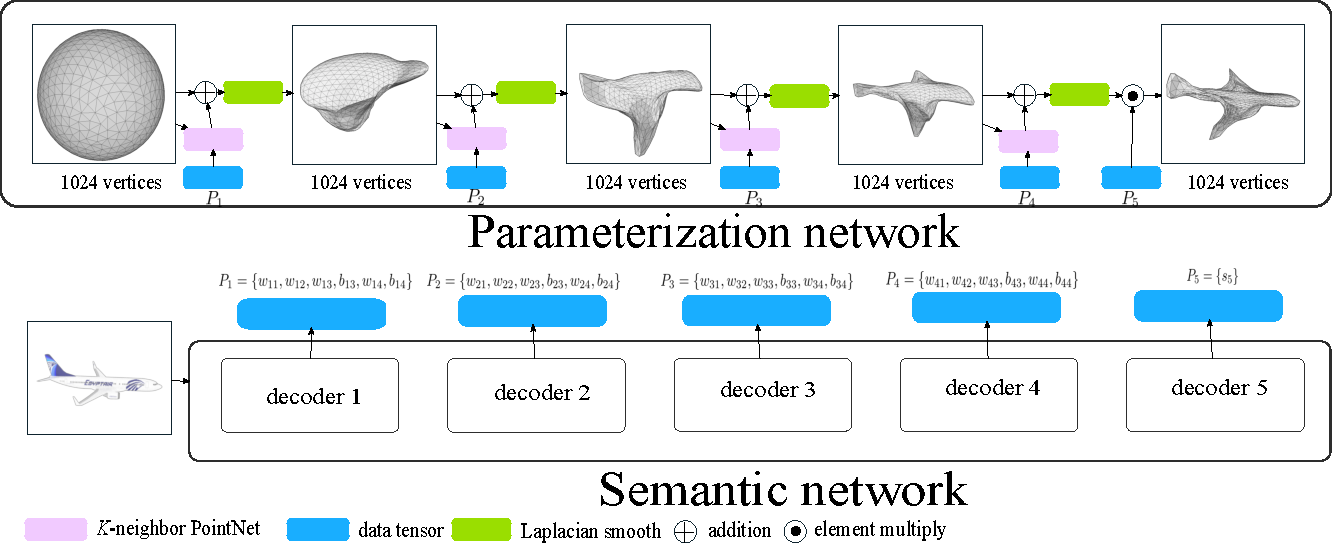
\includegraphics[width=\linewidth]{img/net/overview}
	\caption{The overview of the network: The proposed network consists of two sub-networks. One is the parameterization network that maps points sampled from a unit sphere surface to target shape. The other is the semantic network that takes image as input and predict parameters for the parameterization network. In the figure two version of implementation of parameterization network is shown. Comparing to $\alpha$ version, the $\beta$ version starts with fewer point samples and the point number is increased by mesh-based upsampling in the following layers}
	\label{fig:overview}
\end{figure}
Our original idea about network of \emph{parameterization prediction} was to use a semantic network that takes image as input to predict a mapping from the parameter domain to the target surface. In the proposed framework shown in Figure~\ref{fig:overview}, the mapping is actually expressed by the parameterization network. Instead of directly predicting the mapping, the semantic network predicts parameters for the parameterization network, making the entire network end-to-end trainable.

The parameterization network is built by stacking several \textit{K}-neighbor PointNet (explained in Sec~\ref{subsec:k-n_point_net}). Each \textit{K}-neighbor PointNet takes point set as input and predicts a offsets for each point and add them to the input points. In this way, the parameterization network can map/deform a randomly sampled point set to target shape. By using different randomly generated samples from the parameter domain in the training iterations, the parameterization network can learn to handle the \textit{sampling variation} that is introduced by using specific point set as ground truth. 

The semantic network is built on convolution, deconvolution and fully connected layers, it takes image as input to predict the parameter for the parameterization network. In this way, the semantic network relates the input image to the parameterization.
\subsection{Parameter Domain}
We use unit sphere surface as parameter domain. From the parameter domain, $N$ points are sampled uniformly 
\subsection{\textit{K}-neighbor PointNet for parameterization network} 
\label{subsec:k-n_point_net}
\begin{figure}[htbp]
	\centering
	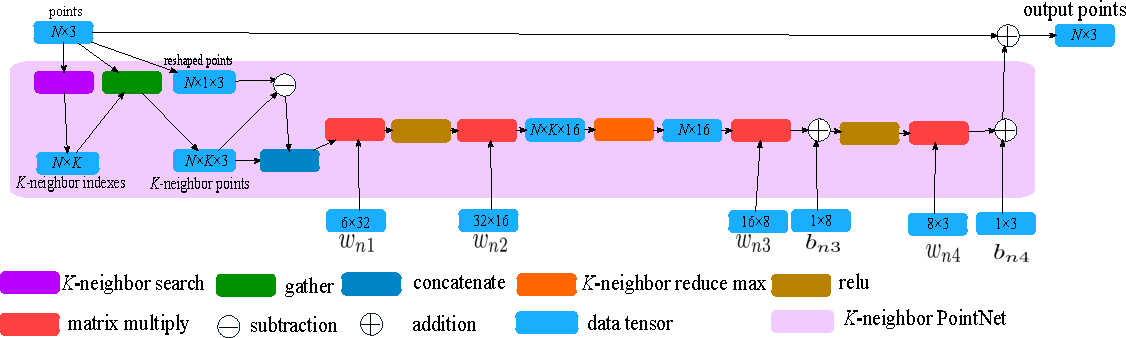
\includegraphics[width=\linewidth]{img/net/k-n_pointnet}
	\caption{The structure of \textit{K}-neighbor PointNet: }
	\label{fig:knpointnet}
\end{figure}
An essential building block for our parameterization network is K-neighbor PointNet. Figure~\ref{fig:knpointnet} shows the internal structure of K-neighbor PointNet. The proposed structure is inspired by and named after PointNet\citep{PointNet} and its follow-up PointNet++\citep{NIPS2017_7095}. K-neighbor PointNet is a network forged with the symmetric functions and apply it on each k-neighbor of input point set to predict a drift for the center of these k-neighborhoods. We propose such structure for two reasons. Firstly, we tried to forge the parameterization network as multi-layer perception network and failed to train it to output any meaningful result. Secondly, we propose such structure after consider human activity. When a potter crafting something from a lump of clay, she do it by applying a serious of squeeze. Each squeeze only affect the clay locally, but all the squeeze together turn the clay into graceful shape. Our parameterization network is designed to simulating such serial local process. 
%\subsection{Mesh based upsampling}
%The building block used in the $\beta$ version of the parameterization network.
\subsection{Laplacian smooth layer}
Another essential building block for our parameterization network is the Laplacian smooth layer. The Laplacian smooth layer applys the mesh based Laplacian smooth for each point in the point set as in (\ref{equ:lpl}). The mesh is constructed by triangulation on the parameterization domain (i.e. the unit sphere surface). In (\ref{equ:lpl}), $\mathcal{N}(\mathbf{x})$ represents the one-ring neighborhood of $\mathbf{x}$. As described in (\ref{equ:lpl}), the Laplacian smooth is a local linear operation and therefore differentiable.
\begin{equation}
\mathbf{x} = \frac{1}{|\mathcal{N}(\mathbf{x})|}\sum_{\mathbf{y}\in\mathcal{N}(\mathbf{x})}\mathbf{y}
\label{equ:lpl}
\end{equation}
The Laplacian smooth layer significantly improves the regularity of the generated shape.
\subsection{Semantic network}
\label{subsec:semnet}
\begin{figure}[htbp]
	\centering
	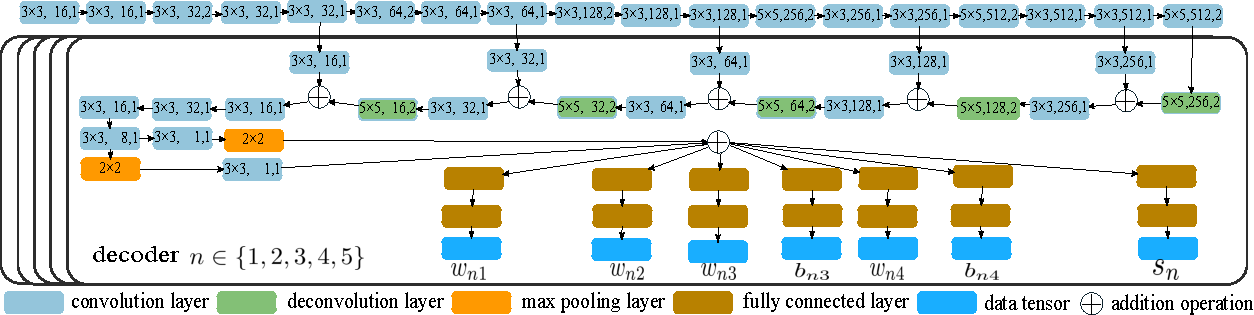
\includegraphics[width=\linewidth]{img/net/semnet}
	\caption{Semantic network: The semantic network takes image as input and predict parameters for the \textit{K}-neighbor PointNet and the global scale operation in the parameterization network. The semantic network have separate decoders for each \textit{K}-neighbor PointNet and and the global scale operation.}
	\label{fig:conv}
\end{figure}
In our semantic network, we use convolution layers to extract semantic features from input image. In order to encode the \textit{semantic variation}, a random feature mapped from the normal distributed random vector is concatenated to the semantic feature.  Figure~\ref{fig:conv} shows the detailed structure for this part. 
\subsection{Losses}
\noindent{\textbf{Chamfer Loss}} The Chamfer distance is directly borrowed from \citep{PSGN}. This loss can drive the output point set to approach the target, but it is not sufficient for a smooth and  
\begin{equation}
l_c = \sum_\mathbf{x} \min||\mathbf{x}-\mathbf{y}||_2^2+\sum_\mathbf{y} \min||\mathbf{x}-\mathbf{y}||_2^2
\end{equation}

\noindent{\textbf{Regularization}}
Edge variation regularization 
idealy if the surface is covered with 

